\documentclass{article}
\usepackage{graphicx}
\usepackage{amsmath,cite}
\usepackage{amsthm}
\usepackage{tikz}
\usetikzlibrary{arrows}

\renewcommand{\arraystretch}{1.5}
\newtheorem{mydef}{Definition}

\title{Solving small shogi}
\author{I. van Duijn \\ Utrecht University}
\begin{document}
\maketitle

\section*{Abstract}
%TODO

\section{Introduction}
Ever since the early days of modern computers there has been great interest in chess programming~\cite{shannon1950xxii}. Initial
focus in the west was mainly on chess and checkers, but when computers were well established in Japan, researchers there adopted
many techniques from computer chess and applied them to their local chess variant, shogi.

\subsection{Shogi}
Shogi (Japanese chess) is a game similar to western chess. It is played on a $9 \times 9$ board and every
player has 20 pieces, some of which correspond to western pieces and others are slightly different.
Black makes the opening move and both players aim to capture the opponent's king.
The main difference between shogi and chess is the so called drop rule.
A piece that is captured by a player now belongs to him and can be placed on \textit{any} vacant square in one of his subsequent turns
(in stead moving a piece already on the board).
Additionally, in shogi nearly all pieces can promote upon moving to or from the promotion zone (starting ranks of opponent).
Unlike western chess, each type of shogi piece can only promoted to one specific piece (e.g. bishop always promotes to a dragon horse).
The drop rule, and to a lesser extent the promotion rule, dramatically increase the game tree complexity of shogi as compared to chess, see Table
\ref{table:complex} for a comparison.\\
\begin{table}
\center
\begin{tabular}{l l l l}
 & Chess & Shogi & Go \\ \hline
State-space complexity & $10^{43}$ & $10^{71}$ & $10^{172}$ \\
Game-tree complexity & $10^{123}$ & $10^{226}$ & $10^{360}$ \\ \hline
\end{tabular}
\caption{The complexities of chess, shogi and go}
\label{table:complex}
\end{table}

\subsection{Computer shogi}
Like computer chess, computer shogi is an active field of research~\cite{iida2002computer}. The main interest is how we can program computers 
such that their play peers with -- and eventually even surpasses -- human professional players. Shogi, being complexer
than western chess, has a game tree too large to make exhaustive search even near feasible. Consequently, research
focusses on clever ways to search the game tree in order to find a good heuristic. Many techniques from computer chess
have been employed, but the drop rule introduced such a novelty that new shogi-specific techniques had to be developed.\\

Unlike in western chess, end game situations
in shogi are not significantly less complex than mid game situations. In fact, any board configuration resulting from the standard
starting setup has exactly 40 pieces in play. Because of this there is no database with solved end games for shogi.
However, in shogi, so called mating problems \footnote{On a predesigned setup, black (lacking a king) can only make checking moves},
which resemble end game situations, are extensively studied ~\cite{grimbergen1999survey}. There exist several
programs that can completely solve a lot of these problems, some of which are quite large~\cite{seo2001pn}. Unfortunately solutions to these shogi
mating problems are not the equivalent of solutions to western chess end games; in shogi, such a solution cannot be directly applied to find a winning move.
However, since the methods used to prove the shortest mating sequence are exact and not heuristical, they or similar methods might be useful to prove
certain subsets or small variants of shogi.\\

\subsection{Solving small shogi variants}
Even though end game situations in shogi are quite complex, there are of course enough situations advanced enough -- near victory -- that they
be perfectly solvable. For instance if no move of the losing player can check the opposing king, it might be possible to restrict the search
for the optimal move to a subset of the board. We are going to emulate this by actually looking at shogi variants played on a smaller board
altogether.

One particular method, proof-number search, has been proved to be quite effective, even outperforming $\alpha\beta$-search~\cite{van2008proof} in
proving the game theoretical value of a game tree. This method has also been succesfully applied to shogi mating
problems~\cite{seo2001pn}~\cite{ueda2008weak}~\cite{sakuta2001performance}. We will discuss the viability of using proof-number search to solve variants of shogi and will test
this method on small shogi variants.

\subsection{Contents}
TODO: introduce all sections.

\section{Method}
We are dealing with generic small sized shogi variants, so representation and algorithms employed have to be sufficiently generic as well.
A small shogi variant is defined by the size of the board, the initial configuration of black (white's is $180^{\circ}$ rotationally symmetrical) and
the size of the promotion zone. The initial configuration consists of a set of pieces, each of which has one or two move sets (taking into account
promotion). Any algorithm that aims to prove the game theoretical value of a variant then only has to have access to two functions based on this
definition: a move generator which can map positions to a set of successing positions, and an evaluation function which recognises terminal
positions and computes their value.

\subsection{Representation}
As stated before, we have to be able to generically represent board positions. A well known technique in computer chess, bitboards, has been
shown~\cite{grimbergen2007using} to be fairly effective in shogi as well. A bitboard is a bit pattern of (at least) the size of the board,
in which each bit encodes some information (e.g. if it is occupied) about the corresponding square. Since the size of the bit pattern can
easily be increased to accomodate larger boards, they are well suited for our purpose. Also, as will be explained later, they allow for easy
generic move generation.

In the current implementation, a position is represented by one bitboard per player per piece's move set (unpromoted and promoted), plus an additional
bitboard per player containing the pieces in hand. Each bitboard corresponding to a certain piece's move set represents all pieces of that type
owned by a specific player. For an $n \times m$ board, each bitboard is fitted in the smallest $nm \leq 2^k$-bit integer (for small
variants $16$ or $32$ bit integers suffice). %TODO: example

To generate moves, we essentially need two things. We need to know for each individual piece where it is, and where it can move to in its current state.
The location of each individual piece can easily be extracted from the bitboards representing a position. To determine where it can move to, a table
is generated which maps position bitboards to move bitboards. %TODO illustrate with example

Finally, the evaluation function can use the move generator to check whether any move captures the opponent's king. Note that the evaluation function
does not give a heuristical value, it only evaluates terminal positions to nonzero values ($1$ for win and $-1$ for loss).

With the move generator and the evaluation function in place, we have an implicit definition of the game tree. The main problem of proving the game
theoretical value efficiently is only generating relevant parts of the tree.

\subsection{Proof-number Search}
Proof-number search~\cite{allis1994proof} is an algorithm designed to find the game theoretical value of a game tree, or more specifically an AND/OR tree.
The tree consists of a root, internal nodes and leaf nodes. Each node is either an AND (white to move) or an OR (black to move) node. By definition, a leaf
node represents one player's victory and thus it has a nonzero value of $1$ (black won) or $-1$ (white won). As in the minmax algorithm, an internal
node's value can be computed by taking the maximum or minimum of the children's value for AND and OR nodes respectively (Figure \ref{tree:simple}).

\begin{figure}[h]
\center
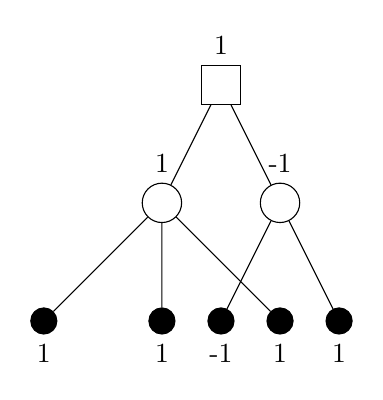
\begin{tikzpicture}[
    all/.style={minimum width=.5cm, minimum height=.5cm},
    and/.style={all, circle, draw},
    or/.style={all, rectangle, draw},
    term/.style={circle, draw=black, fill},
]
    \node [or, label=1] {} 
        child { node [and, label=1] {} 
                child { node [term, label=below:1] {} }
                child { node [term, label=below:1] {} }
                child { node [term, label=below:1] {} }
        }
        child {
            node [and, label=-1] {}
            child { node [term, label=below:-1] {} }
            child { node [term, label=below:1] {} }
        }
    ;
\end{tikzpicture}
\caption{Square AND nodes, circular OR and filled terminal nodes with their respective value.}
\label{tree:simple}
\end{figure}

The most simple form of the minmax algorithm performs a depth-first expansion of the tree to calculate the value of the root. Proof-number search however
expands the tree in a \textit{best-first} manner untill the root can be proved (i.e. determining its game theoretical value). The algorithm starts with a single
unproved node, the root. It then successively picks the most promising unproved node and expands it, i.e. generating its children. Since terminal nodes are proved
directly upon generation, unproved nodes are never terminal nodes and will have children nodes once they are expanded. 

\subsubsection*{Most proving node}
The tree in figure \ref{tree:pnex} has proved ($d$ and $g$) and unproved (the rest) nodes. Since the root $a$ is an OR node, it suffices
to prove either $b$ or $c$. Both these nodes, being AND nodes, need the value of all their children before they can be proved. The sets of
unproved children for $b$ and $c$ respectively are $\{e, f\}$ and $\{h\}$. For the root, in stead of saying that we need to prove
either $b$ or $c$, we can also say we need to prove either $\{e, f\}$ or $\{h\}$. Since the latter set is smaller, it is more
promising trying to prove $c$ than it is to prove $b$. Repeating this argument for determining the most promising branch of the tree
eventually leads to an unproved node, $h$ in the example, which we call the \textit{most proving node}.

\begin{figure}[h]
\center
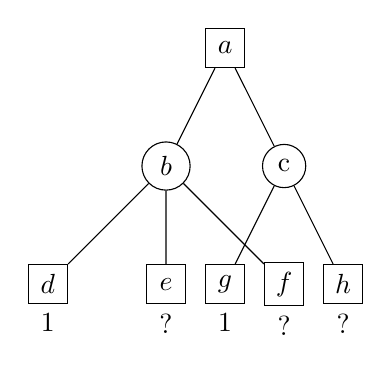
\begin{tikzpicture}[
    all/.style={minimum width=.5cm, minimum height=.5cm},
    and/.style={all, circle, draw},
    or/.style={all, rectangle, draw},
    term/.style={circle, draw=black, fill},
]
    \node [or] {$a$} 
        child { node [and] {$b$} 
                child { node [or, label=below:1] {$d$} }
                child { node [or, label=below:?] {$e$} }
                child { node [or, label=below:?] {$f$} }
        }
        child {
            node [and] {c}
            child { node [or, label=below:1] {$g$} }
            child { node [or, label=below:?] {$h$} }
        }
    ;
\end{tikzpicture}
\caption{Square AND nodes, circular OR, unproved nodes are labelled with a question mark.}
\label{tree:pnex}
\end{figure}

Before we introduce the algorithm, a formal description of the most proving node is required.\\
The \textit{game tree} represents all possible ways to play the game. Whereas the \textit{search tree} is used by the algorithm
and only contains a portion of the game tree relevant for proving the root. The search tree grows as the algorithm expands nodes and
unproved expanded nodes are eventually either proved or disproved.
\begin{mydef}
If a node is proved it has the game theoretical value $1$, indicating a win for the beginning player (Black).
Conversely, if a node is disproved it has value $-1$ and indicates a win for the opponent (White).
An unproved node can be an internal or leaf node of the search tree.
\end{mydef}

To define the most proving node we need a notion of how close a node is of being proved.
\begin{mydef}
Given a search tree $(N, E)$, a set $P \subset N$ is called a proof set of a node $v \in N$ if proving all $w \in P$ will prove $v$.
A disproof set is defined similarly. A (dis)proof set is called minimal if all its subsets are not (dis)proof sets.
\end{mydef}
In the search tree in figure \ref{tree:pnex}, the root has proof sets $\{e, f\}$ and $\{h\}$ of which the latter is minimal,
and minimal disproof sets $\{e, h\}$ and $\{f, h\}$. All supersets of these (dis)proof sets are also (dis)proof sets of course.

For OR nodes, only one of its children has to be proved in order to prove it. Consequently, there exists a set of nodes which is a minimal
proof set for both the parent OR node as well as one of its children. A similar property holds for AND nodes and disproof sets.
\begin{mydef}
Given an unproved OR node $v$ and a subtree $T$ rooted at $w$, then $T$ is called the most promising branch if there exists a set of nodes $P$
which is a minimal proof set of $v$ and $w$. Simalarly if $v$ is an AND node, $T$ is most promising if $P$ is a minimal disproof set.
\end{mydef}
The most proving node is the first unexpanded node the algorithm encounters when successively selecting the most promising branch starting from
the root.

\subsubsection*{(Dis)proof numbers}

\subsubsection*{Breadth-first search}
For comparison there is also a simple breadth-first search implementation.

\subsection{Tree vs. Graph}
So far we have discussed trees and proving nodes to have either value $1$ or $-1$. However there is a third outcome to shogi, draw. Though
very rare in full sized shogi, it can occur on small variants. Draw in shogi occurs if there has been a repitition
of moves four times. Because of the drop rule \textit{any} position on the board can be repeated (repititions), moreover, different move
sequences can lead to the same position (transposition). So strictly adhering to the drawing rule would result in immensely large game trees,
even for the smallest variants.\\
A draw is a forced repitition of moves and as such it does not matter exactly how many repititions are necessary according to the rules,
if one repitition of moves can be forced, any number is possible. If we want to detect these repititons, a history of a position is needed. In trees this
comes natural as there is exactly one path from any node to the root, so reptitions are easily detected. Therefor if we use an actual tree internally
to represent the search tree, we can easily detect repititions and stop the algorithm from searching any deeper than necessary.
To evaluate drawing games we simply run our algorithm twice, the first time repeated positions are a loss for black and the second time for white.
The game is a draw if both runs show that the player who loses on draws also loses the game. Or alternatively, if a player has a winning strategy
even when he loses in potential drawing situations, then that strategy will work regardless of drawing situations.\\

However, even with this modification transpositions %TODO splain why this still does not help


\section{Result}
%subsection: Point out where and why PN fails where BFS succeeds.

%subsection: Elaborate on why PN fails on trees (splosion) and on graphs (algorithm breaks)
%children shogi pns tree: how many nodes/collisions/etc.

\section{Discussion}

\end{document}
